\begin{figure}[p]
\centering
\fbox{\begin{minipage}{.92\linewidth}\small
前129个方向全部从 Wnt3A 与 Dkk4 出发。下图展示前50个方向，以及从 Wnt5 和 Wnt11 出发或指向它们的其他显著方向。
\end{minipage}}
\par\medskip
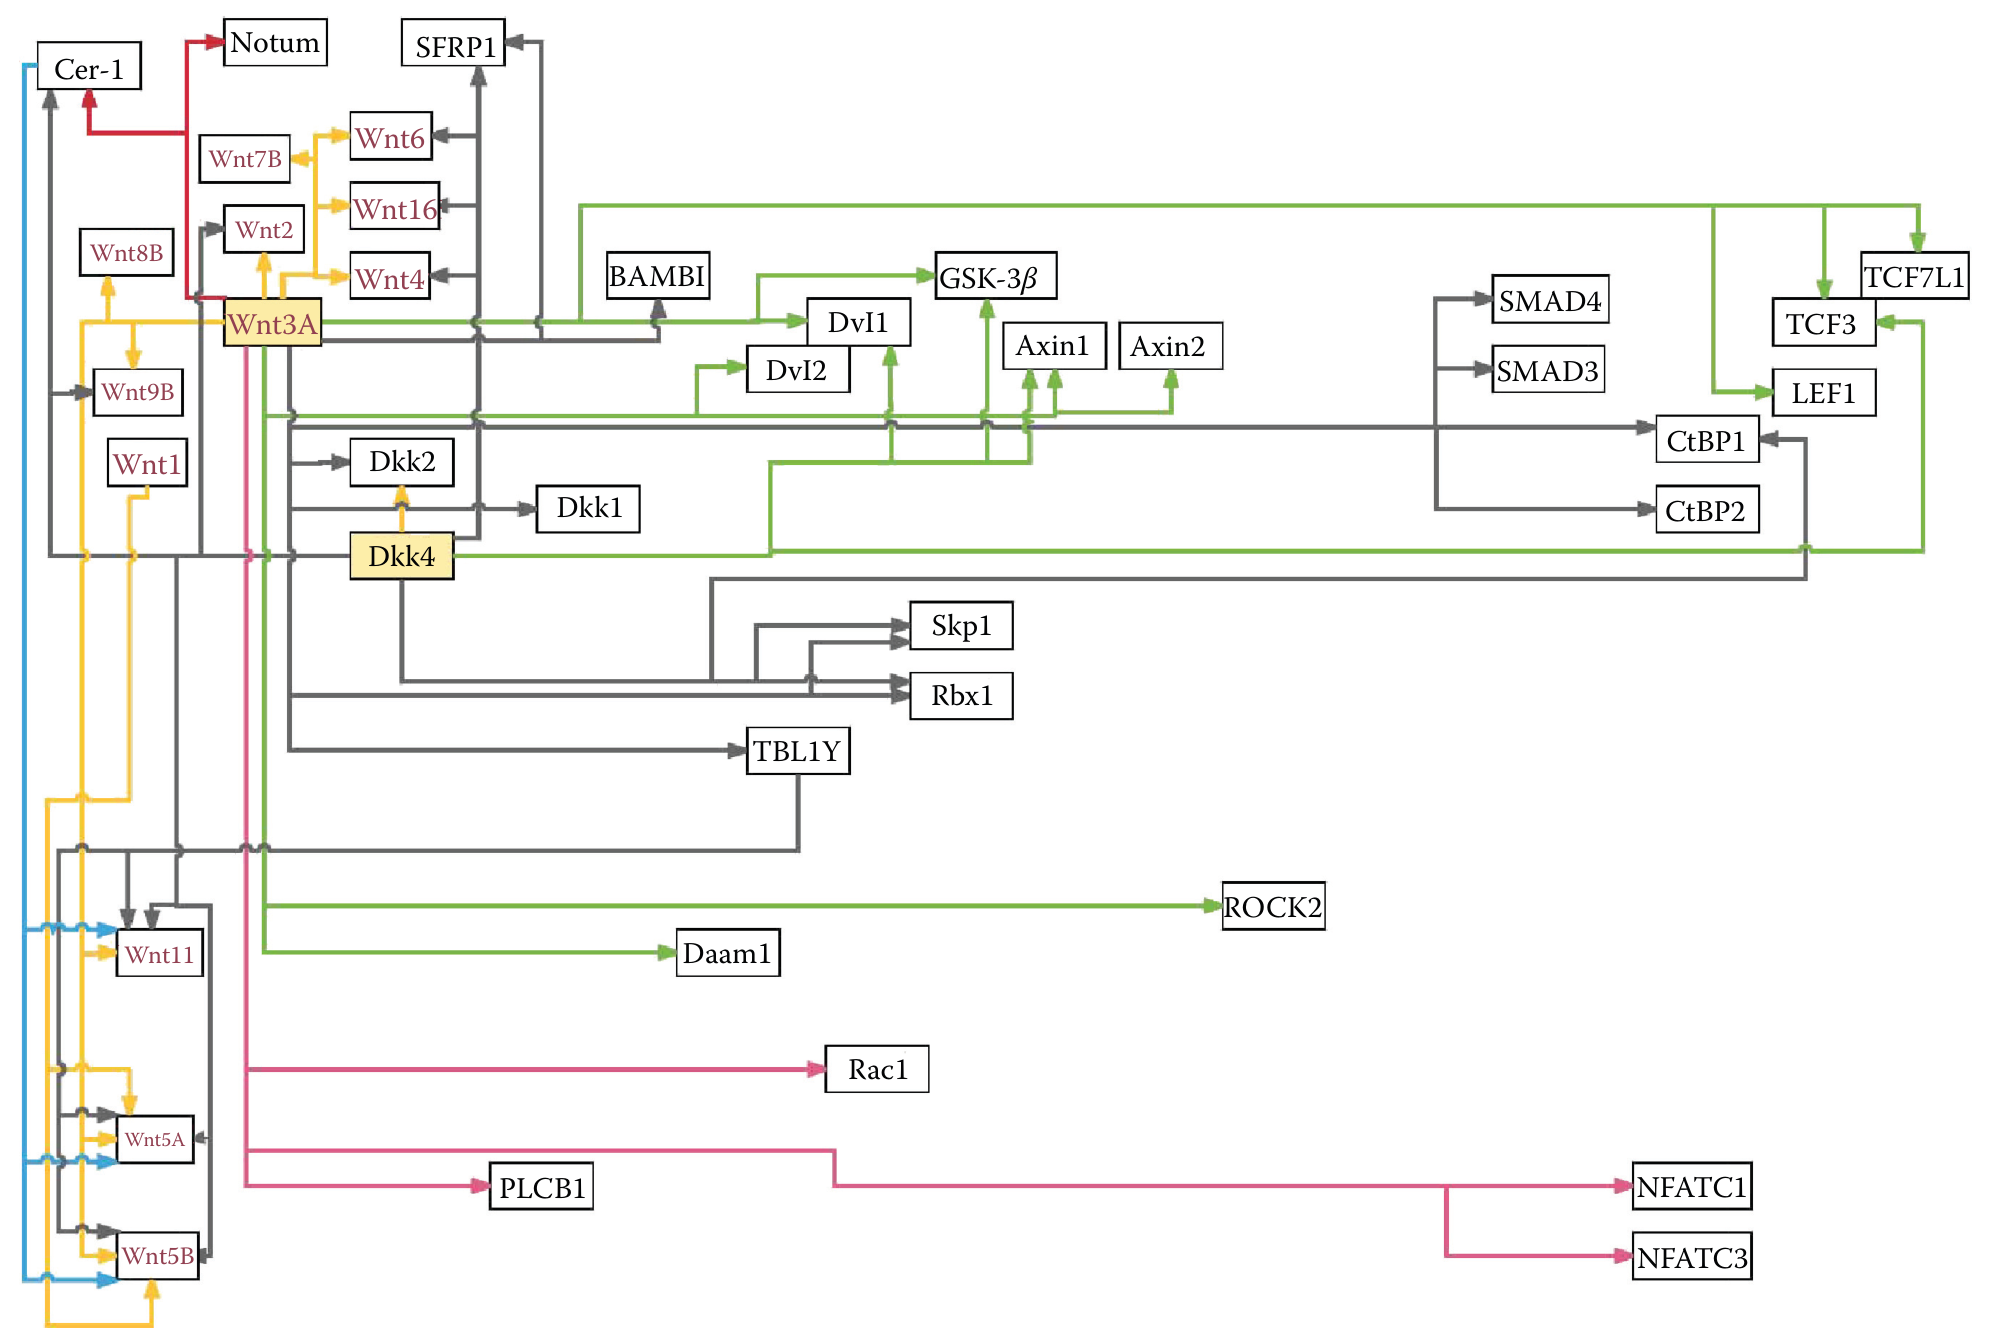
\includegraphics[width=13.8cm]{figures/ch04a_fig25_data.png}
\par\smallskip
\begin{tikzpicture}[x=1cm,y=1cm,font=\footnotesize]
\fill[fill={rgb,255:red,201;green,48;blue,72}] (0,2.10) rectangle (.65,2.32);
\node[anchor=west,inner sep=0] at (.85,2.21) {KEGG 中存在相反方向};
\fill[fill={rgb,255:red,144;green,144;blue,143}] (0,1.68) rectangle (.65,1.90);
\node[anchor=west,inner sep=0] at (.85,1.79) {KEGG 通路中未显示关联};
\fill[fill={rgb,255:red,255;green,198;blue,75}] (0,1.26) rectangle (.65,1.48);
\node[anchor=west,inner sep=0] at (.85,1.37) {存在关联，可据此建立潜在方向};
\fill[fill={rgb,255:red,233;green,88;blue,133}] (0,0.84) rectangle (.65,1.06);
\node[anchor=west,inner sep=0] at (.85,0.95) {KEGG 虚线通路中至少存在一个方向};
\fill[fill={rgb,255:red,119;green,188;blue,67}] (0,0.42) rectangle (.65,0.64);
\node[anchor=west,inner sep=0] at (.85,0.53) {KEGG 实线通路中至少存在一个方向};
\fill[fill={rgb,255:red,89;green,193;blue,224}] (0,0.00) rectangle (.65,0.22);
\node[anchor=west,inner sep=0] at (.85,0.11) {KEGG 中存在直接方向};
\end{tikzpicture}
\origfig{25}{推断得到的 Wnt 信号通路调控网络。}
\label{fig:ch04a-25}
\end{figure}
